\documentclass{stdlocal}
\begin{document}
\section{Quad-Edge Algebra} % (fold)
\label{sec:quad_edge_algebra}

\begin{figure}[H]
  \centering
  \begin{subfigure}[b]{0.4\linewidth}
    \centering
    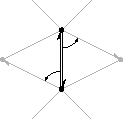
\includegraphics[width=\linewidth]{figures/quad-edge-edge.pdf}
  \end{subfigure}
  \hfill
  \begin{subfigure}[b]{0.4\linewidth}
    \centering
    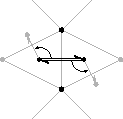
\includegraphics[width=\linewidth]{figures/quad-edge-dual.pdf}
  \end{subfigure}
  \caption[Oriented Quad-Edge Data Structure]{
    \textbf{Oriented Quad-Edge Data Structure}\\
    The figure schematically visualizes all the information a oriented quad-edge stores to access its adjacencies.
    For each edge of the surface, a quad-edge represents both directed edges and both directed dual edges.
    For each directed (dual) edge their origins, represented by vertex or face references, together with pointers to their next counterclockwise neighbore are stored.
  }
  \label{fig:quad-edge}
\end{figure}

\begin{figure}[H]
  \centering
  \begin{subfigure}[b]{0.31\linewidth}
    \centering
    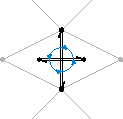
\includegraphics[width=\linewidth]{figures/quad-edge-rot.pdf}
  \end{subfigure}
  \hfill
  \begin{subfigure}[b]{0.67\linewidth}
    \centering
    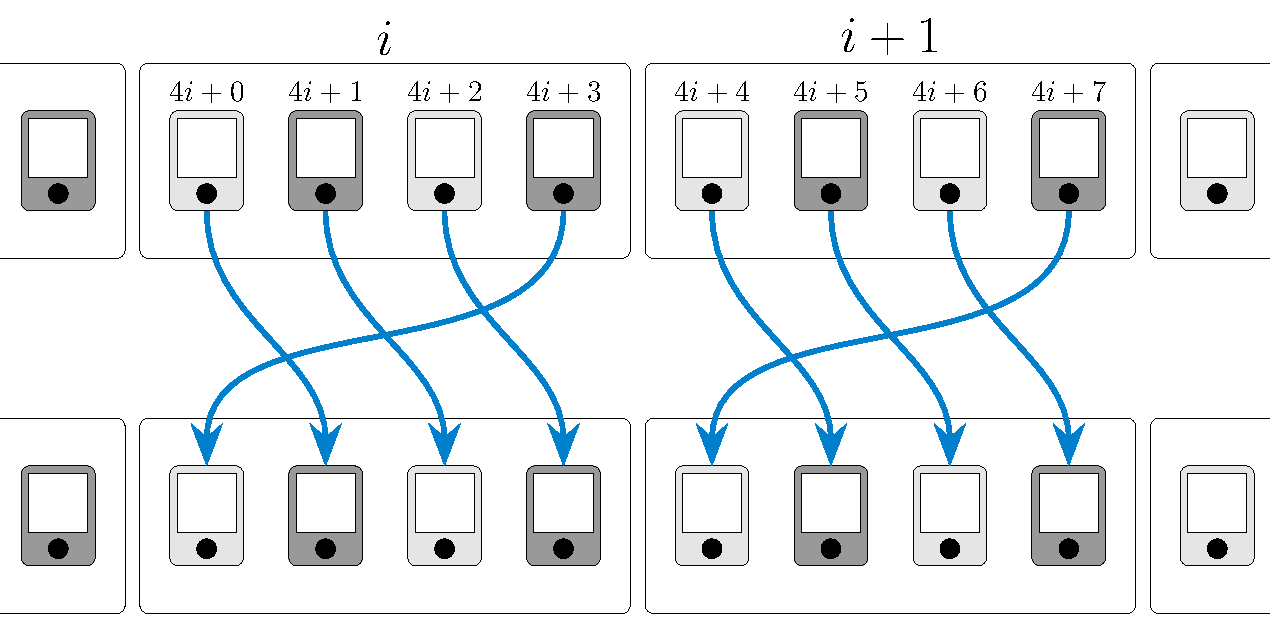
\includegraphics[width=\linewidth]{figures/quad-edge-struct-rot.pdf}
  \end{subfigure}
  \caption[Oriented Quad-Edge Rotation]{
    \textbf{Oriented Quad-Edge Rotation}\\
    The counterclockwise rotation of a quad-edge allows to easily switch between the graph and the dual graph of a surface.
    % Using bit masks, it can be implemented by adding $1$ to the
  }
  \label{fig:quad-edge-rotation}
\end{figure}

\newpage
\inputCodeBlock[title = Quad-Edge Algebra]{code/quad-edge-algebra.hpp}

% section quad_edge_algebra (end)
\end{document}
